\documentclass[10pt]{beamer}
% \documentclass[handout,10pt]{beamer}
\usepackage{my_style}
%%%%%%%%%%%%%%%%%%%%%%%%%%%%%%%%%%%%%%%%%%%%%%%%%%%%%%%%%%%%%%%%%%%%%%%%
%%%%%%%%%%%%%%%%%%%%%%%%%%%%%%%%%%%%%%%%%%%%%%%%%%%%%%%%%%%%%%%%%%%%%%%%

\title[Math/CS 375]{Lecture 14 - A}
\subtitle{\S 8.2 Singular Value Decomposition }

\begin{document}
% -------------------------------------------------
\begin{frame}
  \titlepage
\end{frame}

%%%%%%%%%%%%%%%%%%%%%%%%%%%%%%%%%%%%%%%%%%%
\begin{frame}{Goals}
We will answer these questions:\\[3mm]
\begin{itemize}
    \item What are singular values and why are they more versatile than eigenvalues?
    \item How do you find the singular value decomposition?
    \item What is an overdetermined system and when does it arise in applications?
    \item What is the standard way to solve an overdetermined system?
    \item How can you use the SVD to solve overdetermined systems and why would you want to?
\end{itemize}
\end{frame}
%%%%%%%%%%%%%%%%%%%%%%%%%%%%%%%%%%%%%%%%%%%%%%%%%%%%%%%%%%%%%%%%%%%%%%%%
\sectionframe{Linear Algebra Review}
%%%%%%%%%%%%%%%%%%%%%%%%%%%%%%%%%%%%%%%%%%%%%%%%%%%%%%%%%%%%%%%%%%%%%%%%

\begin{frame}{Matrix Multiplication $C = AB$}{Column Views}

The product $C = AB$ can be viewed by columns

\begin{block}{Column View}
Each column of \( C \) is the product of \( A \) with the corresponding column of \( B \):
$$\text{Col}_j(C) = A \cdot \text{Col}_j(B)$$
\end{block}
\begin{align*}
\begin{bmatrix}
    | &  & | \\
    c_1    & \dots  & c_n \\
    | &   & |
\end{bmatrix} &= A
\begin{bmatrix}
    | &  & | \\
    b_1    & \dots  & b_n \\
    | &   & |
\end{bmatrix}\\
c_j &= A b_j 
\end{align*}

\vspace{3mm}
\begin{center}
    \emph{This will be useful later.}
\end{center}
\end{frame}

%%%%%%%%%%%%%%%%%%%%%%%%%%%%%%%%%%%%%%%%%%%%%%%%%%%%%%%%%%%%%%%%%%%
\begin{frame}{Multiply by $e_i$}

\begin{itemize}
    \item Let $I$ be an $n\times n$ identity matrix 
        $$
        I = \begin{bmatrix}
            1 & 0 & 0\\
            0 & 1 & 0\\
            0 & 0 & 1
        \end{bmatrix}
        $$

    \item We define $e_i$ to the $i^{th}$ column of $I$

    \item Consider the multiplication $Ae_1$
    \begin{align*}
        Ae_1 = \begin{bmatrix}
            a & b & c\\
            d & e & f\\
            g & h &i
        \end{bmatrix} \begin{bmatrix}
            1\\0 \\0
        \end{bmatrix} = \begin{bmatrix}
            a \\ d \\ g
        \end{bmatrix}
    \end{align*}

    \begin{block}{General Formula}
    
    $$
    A e_i = a_i,
    $$
    where $a_i$ is the $i^{th}$ column of $A$
    \end{block}
\end{itemize}
    
\end{frame}

%%%%%%%%%%%%%%%%%%%%%%%%%%%%%%%%%%%%%%%%%%%%%%%%%%%%%%%%%%%%%%%%%%%

\begin{frame}{Eigenvalues, Eigenvectors}

    \define{Eigenvalues and Eigenvectors}{
    For a matrix $A$, the scalar-vector pairs ($\lambda$, $v$) such that
    \[Av=\lambda v, \qquad v \neq 0\] are \textbf{eigenvalue-eigenvectors}.     
    }

\begin{itemize}

\item To find the eigenvalues, we find the roots of the \textbf{characteristic polynomial}
$$p(\lambda) := \det(\lambda I - A)$$

\item We can only find eigenvalues for \emph{square matrices}

\end{itemize}
\end{frame}

%%%%%%%%%%%%%%%%%%%%%%%%%%%%%%%%%%%%%%%%%%%%%%%%%%%%%%%%%%%%%%%%%%%%%%%%
% \begin{frame}{Eigenvalues}
% Assume that 
% $$ A v = \lambda v$$
% for $v\neq 0$. 

% \vspace{4mm}

% \begin{block}{Some Properties}
%     \begin{itemize}
%         \item $A^k v = \lambda^k v$
%         \item $1/\lambda$ is an eigenvlaue of $A^{-1}$
%         \item If $A=A^T$ (and real) then all of its eigenvalue are real
%         \item If $P$ is invertible, then $A$ and $P A P^{-1}$ have the same eigenvalues
%     \end{itemize}
% \end{block}

% % {
% % \define{Similarity}{Matrices $A$ and $B$ are \textbf{similar} if there is an invertible matrix $P$ such
% % that
% % \[
% % P^{-1} B P = A
% % \]
% % }
% % }
    
% \end{frame}

%%%%%%%%%%%%%%%%%%%%%%%%%%%%%%%%%%%%%%%%%%%%%%%%%%%%%%%%%%%%%%%%%%%%%%%%

% \begin{frame}{Similarity}
% \begin{theorem}
%     If $A$ and $B$ are similar matrices then they have the same eigenvalues.
% \end{theorem}
% Proof: 

% \begin{itemize}
%     \item  Let $v,\lambda$ be an eigenvector, eigenvalue pair for matrix $B$.  
%     \item We use the assumption $P^{-1} B P = A$
% \begin{align*}
%   B v & = \lambda v, \quad v\neq 0\\
%   P A P^{-1} v &= \lambda v\\
%   A P^{-1} v &= \lambda P^{-1} v\\
%   A w   &= \lambda w, \quad w\neq 0.
% \end{align*}
% \item Thus, $w=P^{-1} v$ is an eigenvector of $A$ with the same eigenvalue $\lambda$.
% \end{itemize}

% \vspace{3mm}
% \begin{center}
%     \emph{This will be useful later.}
% \end{center}

% \end{frame}



%%%%%%%%%%%%%%%%%%%%%%%%%%%%%%%%%%%%%%%%%%%%%%%%%%%%%%%%%%%%%%%%%%%%%%%%
\begin{frame}{Orthogonal Matrix}

{
\define{Orthogonality}{
    A square matrix $U$ is \textbf{orthogonal} if $U^T U = U U^T = I$.
}
}
\vspace{3mm}

\begin{block}{Some Properties}
\begin{itemize}
    \item Each row and column of $U$ has norm 1
    \item The columns of $U$ are an orthonormal set of vectors 
    \item The rows of $U$ are an orthonormal set of vectors 
    \item $U^{-1}= U^T$
    \item They are norm preserving: $\| U v \| = \|v\|$
\end{itemize}
\end{block}

\begin{center}
    \emph{This will be useful later.}
\end{center}
\end{frame}

%%%%%%%%%%%%%%%%%%%%%%%%%%%%%%%%%%%%%%%%%%%%%%%%%%%%%%%%%%%%%%%%%%%%%%
\begin{frame}{Orthogonal Matrix}

\begin{block}{Example}
    Consider the matrix 
    $$A=
    \begin{bmatrix}
        0 & -1\\ 1 & 0
    \end{bmatrix}
    $$
\end{block}
\begin{itemize}
    \item The inverse is 
    $$
    A^{-1} = \begin{bmatrix}
        0 & 1\\ -1 & 0
    \end{bmatrix} = A^T
    $$

    \item If we let $x = \begin{bmatrix}
        3&4
    \end{bmatrix}^T$, then
    $$
        \| Ax\| = \left\| \begin{bmatrix}
            0 &  -1\\
            1 & 0
        \end{bmatrix} \begin{bmatrix}
            3\\4
        \end{bmatrix}\right\|= \left\| \begin{bmatrix}
            -4\\3
        \end{bmatrix}\right\| = \|u\|  
    $$
    \item The matrix $A$ is orthogonal
    
\end{itemize}
    
\end{frame}

%%%%%%%%%%%%%%%%%%%%%%%%%%%%%%%%%%%%%%%%%%%%%%%%%%%%%%%%%%%%%%%%%%%%%%

% \begin{frame}{Gram-Schmidt orthogonalization}

% \method{Gram-Schmidt}{Set of vectors $\{a_1, a_2, ..., a_n\}$}{Ortho-normalized vectors $\{q_1, q_2, ..., q_n\}$ }{Adjust the vectors so they are all orthogonal to each other, and have unit length}
% \begin{itemize}

% \item Let $A = [a_1| a_2 | \cdots |a_n]$. First normalize $a_1$ and obtain $$q_1 = \frac{a_1}{||a_1||} = \frac{a_1}{r_{11}}.$$  Now subtract from $a_2$ the components from  $q_1$.  This is given by $$a_2' = a_2 - (q_1^Ta_2)q_1 = a_2 - r_{12} q_1.$$  

% \item Normalizing $a_2'$ we have $$q_2 = \frac{a_2'}{||a_2'||} = \frac{a_2'}{r_{22}}$$

% \item Repeat recursively $a_i' = a_i - (q_{i-1}^Ta_i)q_{i-1}$, then $q_i = a_i'/|| a_i'||$.
% \end{itemize}
% \end{frame}

%%%%%%%%%%%%%%%%%%%%%%%%%%%%%%%%%%%%%%%%%%%%%%%%%%%%%%%%%%%%%%%%%%%%%%%%

\begin{frame}{Limitations of Eigenvalues}
\begin{itemize}

    \item Image files are actually matrices 
    
    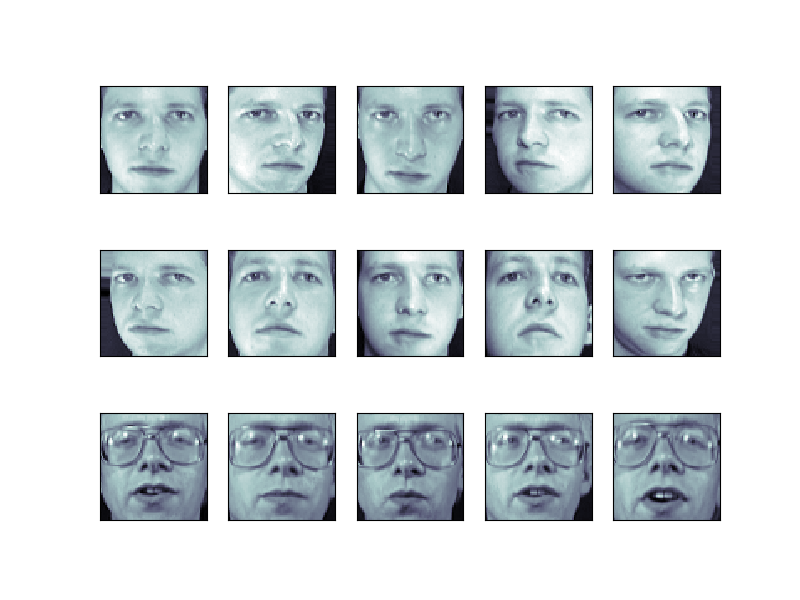
\includegraphics[scale=0.25]{figs/eigenfaces.png}

    \item Eigenvalues of images used to be prominent in face recognition\\[3mm]

    \item Similar eigenvalues, eigenvectors $\implies$ similar faces

\end{itemize}
\end{frame}

%%%%%%%%%%%%%%%%%%%%%%%%%%%%%%%%%%%%%%%%%%%%%%%%%%%%%%%%%%%%%%%%%%%%%%%%

\begin{frame}{Limitations of Eigenvalues}
\begin{itemize}
   {\question{
       What if the image was not $n\times n$? Does that mean facial recognition is impossible?
   }}
   \vspace{3mm}

    \item Finding eigenvalues is only possible for $n\times n$ matrices\\[3mm] 

    \item If we can't find eigenvalues, facial recognition is not possible\\[3mm]

    \onslide<2>{
    
    \item However...  $AA^T$ and $A^TA$ are both always square matrices.\\[3mm]
    
    \keyidea{
        Even if an image is rectangular, we can still find the eigenvalues of $AA^T$ which is always a square.
    }
    }
\end{itemize}
    
\end{frame}

%%%%%%%%%%%%%%%%%%%%%%%%%%%%%%%%%%%%%%%%%%%%%%%%%%%%%%%%%%%%%%%%%%%%%%
\sectionframe{Singular Value Decomposition}
%%%%%%%%%%%%%%%%%%%%%%%%%%%%%%%%%%%%%%%%%%%%%%%%%%%%%%%%%%%%%%%%%%%%%%%%
\begin{frame}{Symmetric Matrices}
\begin{itemize}
    \item Consider the rectangular matrix $A$
    $$
        A = \begin{bmatrix}
            1 & 2\\ 3 & 4 \\ 5 & 6
        \end{bmatrix}
    $$
    \item The matrix $AA^T$ is square  
    $$
    A A^T = \begin{bmatrix}
        5 & 11 & 17\\
        11 & 25 & 39\\
        17 & 39 & 61
    \end{bmatrix}
    $$
    \item The matrix $A^TA$ is also square 
    $$
    A^TA = \begin{bmatrix}
        35 & 44\\
        44 & 56
    \end{bmatrix}
    $$
\end{itemize}
\keyidea{Even if $A$ doesn't have eigenvalues, $AA^T$ and $A^TA$ do have eigenvalues.}
\end{frame}

%%%%%%%%%%%%%%%%%%%%%%%%%%%%%%%%%%%%%%%%%%%%
\begin{frame}{Singular Values}

{\define{Singular Values}{
The \textbf{singular values} of an $m\times n$ matrix $A$ are
$$\sigma_1, \sigma_2,\dots,\sigma_r,$$
where $r=\min(m,n)$ and the $\sigma$'s are square roots of the eigenvalues of $A^T A$ or $AA^T$. 
}}

\begin{block}{How to Find Singular Values of $A$}
\begin{enumerate}
    \item Calculate $AA^T$ or $A^TA$ (whichever is smaller).
    \item Find the eigenvalues of that matrix.
    \item Take the square root of those eigenvalues.
\end{enumerate}
    
\end{block}

\end{frame}


%%%%%%%%%%%%%%%%%%%%%%%%%%%%%%%%%%%%%%%%%%%%%%%%%%%%%%%%%%%%%%%%%%%%%
\begin{frame}{Singular Value Example}
\begin{example}
    Find the singular values of 
    $$
    A = \begin{bmatrix}
        1 & 0 \\
        1 & 2\\
        0 & 1
    \end{bmatrix}
    $$
\end{example}

\begin{enumerate}
    \item Calculate $B=A^TA$ since its $2\times 2$
    $$
    B = A^TA = \begin{bmatrix}
        1 & 1 & 0\\
        0 & 2 & 1
    \end{bmatrix}\begin{bmatrix}
        1 & 0\\
        1 & 2\\
        0 & 1
    \end{bmatrix} = \begin{bmatrix}
        2 & 2\\
        2& 2
    \end{bmatrix}
    $$
    \item Find eigenvalues of $B$
    $$
    \det(\lambda B-I) = \begin{vmatrix}
        \lambda-2 & -2\\
        -2 & \lambda - 2
    \end{vmatrix} = \lambda^2 -4\lambda+4-4=\lambda(\lambda-4)=0\implies \lambda=0,4
    $$
    \item Take the square root of the eigenvalues
    $$
    \sigma_1= \sqrt{4}=2,\quad \sigma_2=\sqrt{0}=0
    $$
\end{enumerate}

    
\end{frame}

%%%%%%%%%%%%%%%%%%%%%%%%%%%%%%%%%%%%%%%%%%%%%%%%%%%%%%%%%%%%%%%%%%%%%


\begin{frame}{Singular Value Decomposition (SVD) }


{\define{SVD}{
\textbf{SVD} is the factorization of $A \in \mathbb{R}^{m \times n}$ in the form $A = U S V^T$, 
where $U$ ($m \times m$) and $V$ ($n \times n$) are orthogonal and $S$ ($m
\times n$) is a diagonal matrix containing the \textbf{singular values} of $A$ 
\[
    \underbrace{\sigma_1 \geq \sigma_2 \geq \dots \geq \sigma_r}_{\text{unspecified}} > \underbrace{\sigma_{r+1} = \dots =\sigma_p=0}_{\text{zero}}
\]
where $r=rank(A)$ and $p=min(m,n)$.
}}

\[
A =
\begin{bmatrix}
    | &  & | \\
    u_1    & \dots  & u_m \\
    | &   & |
\end{bmatrix}
\begin{bmatrix}
    \sigma_1 &        &          &        &\\
             & \ddots &          &        & \\
             &        & \sigma_r &        & \\
             &        &          & \ddots & \\
             &        &          &        & 0 
\end{bmatrix}
\begin{bmatrix}
    - & v_1^T & -\\
     & \vdots & \\
    - & v_n^T & -
\end{bmatrix}
\]
\end{frame}

%%%%%%%%%%%%%%%%%%%%%%%%%%%%%%%%%%%%%%%%%%%%%%%%%%%%%%%%%%%%%%%%%%%%%%%%

\begin{frame}{Visualizing the Shapes}{SVD is possible for any size}
\begin{itemize}
    \item If $A$ is a $4 \times 2$ matrix  
\begin{equation*}
A = U S V^T = \begin{bmatrix}
    u_{11} & u_{12}  & u_{13} & u_{14}\\
    u_{21} & u_{22}  & u_{23} & u_{24}\\
    u_{31} & u_{32} & u_{33}  & u_{34}\\ 
    u_{41} & u_{42} & u_{43}  & u_{44}\\ 
\end{bmatrix} \begin{bmatrix}
    \sigma_1 & 0  \\
    0 & \sigma_2  \\
    0 & 0   \\ 
    0 & 0   \\ 
\end{bmatrix} \begin{bmatrix}
    v_{11} & v_{12}\\
    v_{21} & v_{22} \\
\end{bmatrix}^T
\end{equation*}

    \item If $A$ is a $2 \times 3$ matrix 
    \begin{equation*}
A = U S V^T = \begin{bmatrix}
    u_{11} & u_{12} \\
    u_{21} & u_{22}  \\
\end{bmatrix} \begin{bmatrix}
    \sigma_1 & 0 & 0 \\
    0 & \sigma_2  & 0 \\
\end{bmatrix} \begin{bmatrix}
    v_{11} & v_{12} & v_{13} \\
    v_{21} & v_{22} & v_{23} \\
    v_{31} & v_{32} & v_{33}
\end{bmatrix}^T
\end{equation*}

\item $A$ has $p= 2$ singular values $\sigma_1$ and $\sigma_2$

\item If $A$ is rank 1, then $\sigma_2 = 0$

% \method{SVD}{Any matrix A}{Matrices $S$,$U$, and $V$ satisfying $A=USV^T$}{The }

\end{itemize}

\end{frame}

%%%%%%%%%%%%%%%%%%%%%%%%%%%%%%%%%%%%%%%%%%%%%%%%%%%%%%%%%%%%%%%%%%%%%%%%


\begin{frame}{Applications of Singular Values}

\begin{enumerate}
    \item Search Technology: find closely related documents or images 
    \item Clustering: aggregate documents or images into similar groups
    \item Compression: efficient image storage
    \item Principal axis: find the main axis of a solid (engineering/graphics)
    \item Key words: identify best search tags for text
    \item Graphs: partition graphs into subgraphs (graphics, analysis)
    \item \textbf{Least squares}
\end{enumerate}

\end{frame}

%%%%%%%%%%%%%%%%%%%%%%%%%%%%%%%%%%%%%%%%%%%%%%%%%%%%%%%%%%%%%%%%%%%%%%%%

\sectionframe{Calculating the SVD}

\begin{frame}{Calculating the SVD}

\begin{block}{Goal}
For a matrix $A \in \mathbb{R}^{m \times n}$, calculate the decomposition 
    $$A = U S V^T$$
where 
\begin{enumerate}
    \item $S$ is diagonal and contains the singular values of $A$
    \item $U$ is orthogonal 
    \item $V$ is orthogonal 
\end{enumerate}
\end{block}

\vspace{3mm}

\begin{center}
    \emph{Let's derive a formula for each matrix}
\end{center}
\end{frame}
%%%%%%%%%%%%%%%%%%%%%%%%%%%%%%%%%%%%%%%%%%%%%%%%%%%%%%%%%%%%%%%%%%%%%%%%
\begin{frame}{Calculating $S$}{We know that $S$ contains the singular values on the diagonal}

\begin{block}{Steps}
    \begin{enumerate}
        \item Calculate $B = A^T A$ or $B = AA^T$ (choose the smaller one)
        \item Find all eigenvalues of $B$ by solving  
            $$ \det (\lambda I - B) = 0$$
        \item Calculate the square root of the eigenvalues 
            $$ \sigma = \sqrt{\lambda}$$
    \end{enumerate}
\end{block}
$$
S = \begin{bmatrix}
    \sigma_1 &        &          &        &\\
             & \ddots &          &        & \\
             &        & \sigma_r &        & \\
             &        &          & \ddots & \\
             &        &          &        & 0 
\end{bmatrix}
$$
\end{frame}

%%%%%%%%%%%%%%%%%%%%%%%%%%%%%%%%%%%%%%%%%%%%%%%%%%%%%%%%%%%%%%%%%%%%%%%%
\begin{frame}{What is $U$?}{Part 1}
\begin{enumerate}
    \item Begin with the SVD of \( A \):  
        $$ A = U S V^T $$

    \item Next, calculate $AA^T$:
    \begin{align*}
         AA^T &= U S V^T (U S V^T)^T\\
              &= U S V^T VS^TU^T\\
              &= U S (V^T V)S^TU^T\\
              &= U S S^T U^T 
    \end{align*}
        
    \item Therefore, (letting $S^2 := SS^T$) we have  
        $$
        AA^TU = U S^2
        $$
\end{enumerate}
\end{frame}
%%%%%%%%%%%%%%%%%%%%%%%%%%%%%%%%%%%%%%%%%%%%%%%%%%%%%%%%%%%%%%%%%%%%%%%%
\begin{frame}{What is $U$?}{Part 2}

\begin{enumerate}
\setcounter{enumi}{3}
    \item Consider the RHS of $AA^TU = U S^2$ 
        \begin{align*}
        U S^2&=U
\begin{bmatrix}
    \sigma_1^2 &  &  \\
         & \ddots  &  \\
     &   & \sigma_m^2
\end{bmatrix}\\
&=U\begin{bmatrix}
    e_1 \sigma_1 | e_2\sigma_2|\cdots|e_m\sigma_m
\end{bmatrix}\\
&=\begin{bmatrix}
    u_1 \sigma_1 | u_2\sigma_2|\cdots|u_m\sigma_m
\end{bmatrix}\\
\end{align*}
        
\item The column view gives of $AA^TU = U S^2$ is
        $$AA^T u_i = \sigma_i^2 u_i$$
\end{enumerate}
\end{frame}

%%%%%%%%%%%%%%%%%%%%%%%%%%%%%%%%%%%%%%%%%%%%%%%%%%%%%%%%%%%%%%%%%%%%%%%%
\begin{frame}{What is $U$?}{Part 3}

{\question{What is the significance of this equation? $$AA^T u_i = \sigma_i^2 u_i$$
}}

\begin{align*}
    &\underbrace{AA^T}_{\text{matrix}} &\underbrace{u_i}_{\text{vector}} &&=& &\underbrace{\sigma_i^2}_{\text{scalar}} &&\underbrace{u_i}_{\text{same vector}}&&\\
    \onslide<2>{ &B &v &&=&  &\lambda &&v& &}
\end{align*}

\onslide<2>{
\keyidea{The columns of $U$ are the eigenvectors of $AA^T$!}
}

\end{frame}
%%%%%%%%%%%%%%%%%%%%%%%%%%%%%%%%%%%%%%%%%%%%%%%%%%%%%%%%%%%%%%%%%%%%%%%%
\begin{frame}{Calculating \( U \)}{Steps to find the left singular vectors}

\begin{block}{Steps}
    \begin{enumerate}
        \item Compute \( B = AA^T \), ensuring \( B \in \mathbb{R}^{m \times m} \).
        \item Solve the eigenvalue equation for \( B \):  
            $$ \det (\lambda I - B) = 0 $$  
            to find the eigenvalues \( \lambda_1, \lambda_2, \dots, \lambda_m \).
        \item Compute the eigenvectors of \( B \), denoted as \( \mathbf{u}_1, \mathbf{u}_2, \dots, \mathbf{u}_m \).
        \item Normalize each eigenvector:  
            $$ \mathbf{u}_i = \frac{\mathbf{u}_i}{\|\mathbf{u}_i\|} $$
        \item Form \( U \) as the matrix with these normalized eigenvectors as columns:
            $$ U = \begin{bmatrix} \mathbf{u}_1 & \mathbf{u}_2 & \cdots & \mathbf{u}_m \end{bmatrix} $$
    \end{enumerate}
\end{block}



\end{frame}
%%%%%%%%%%%%%%%%%%%%%%%%%%%%%%%%%%%%%%%%%%%%%%%%%%%%%%%%%%%%%%%%%%%%%%%%
\begin{frame}{What is $V$?}
\begin{enumerate}
    \item The SVD of \( A \):  
        $$ A = U S V^T $$
        implies:  
        $$ A^TA = (U S V^T)^TU S V^T  = V  S^T S V^T $$
        
    \item Therefore, (letting $S^2 := S^TS$) we have  
        $$ A^TAV = V S^2$$
        
    \item The column view gives us 
        $$A^TA v_i = \sigma_i^2 v_i$$
    \item \emph{By definition}, $v_i$ is an eigenvector for $A^TA$
\end{enumerate}
\end{frame}

%%%%%%%%%%%%%%%%%%%%%%%%%%%%%%%%%%%%%%%%%%%%%%%%%%%%%%%%%%%%%%%%%%%%%%%%
\begin{frame}{Calculating \( V \)}{Steps to find the right singular vectors}

\begin{block}{Steps}
    \begin{enumerate}
        \item Compute \( B = A^T A \), ensuring \( B \in \mathbb{R}^{n \times n} \).
        \item Solve the eigenvalue equation for \( B \):  
            $$ \det (\lambda I - B) = 0 $$  
            to find the eigenvalues \( \lambda_1, \lambda_2, \dots, \lambda_n \).
        \item Compute the eigenvectors of \( B \), denoted as \( \mathbf{v}_1, \mathbf{v}_2, \dots, \mathbf{v}_n \).
        \item Normalize each eigenvector:  
            $$ \mathbf{v}_i = \frac{\mathbf{v}_i}{\|\mathbf{v}_i\|} $$
        \item Form \( V \) as the matrix with these normalized eigenvectors as columns:
            $$ V = \begin{bmatrix} \mathbf{v}_1 & \mathbf{v}_2 & \cdots & \mathbf{v}_n \end{bmatrix} $$
    \end{enumerate}
\end{block}

\end{frame}
%%%%%%%%%%%%%%%%%%%%%%%%%%%%%%%%%%%%%%%%%%%%%%%%%%%%%%%%%%%%%%%%%%%%%%%%


\begin{frame}{Summary on  $A=USV^T$}
\[
A =
\underbrace{
\begin{bmatrix}
    | &  & | \\
    u_1    & \dots  & u_m \\
    | &   & |
\end{bmatrix}}_{\textrm{eigenvectors of}\; AA^T}
\underbrace{
\begin{bmatrix}
    \sigma_1 &        &          &        &\\
             & \ddots &          &        & \\
             &        & \sigma_r &        & \\
             &        &          & \ddots & \\
             &        &          &        & 0 
\end{bmatrix}}_{\textrm{eigenvalues of both}}
\underbrace{
\begin{bmatrix}
    - & v_1^T & -\\
     & \vdots & \\
    - & v_n^T & -
\end{bmatrix}}_{\textrm{eigenvectors of}\; A^TA}
\]
\begin{enumerate}
\item Compute $A^TA$ 
\item Find the eigenvalues of $A^TA$ (these are $\sigma_i^2$) 
\item Find the orthonormal eigenvectors of $A^TA$ (these are the rows of $V^T$) 
\item Compute  $AA^T$ 
\item Find the orthonormal eigenvectors of $AA^T$ (these are the columns of $U$)
\end{enumerate}

\end{frame}



\begin{frame}{Example}
\begin{example}
Find the SVD of 
\[
A = \begin{bmatrix}2 & -2\\ 1 & 1\end{bmatrix}
\]
\end{example}
First construct $A^T A$:
\[
A^TA 
= 
\begin{bmatrix}2 & 1\\ -2 & 1\end{bmatrix}
\begin{bmatrix}2 & -2\\ 1 & 1\end{bmatrix}
=
\begin{bmatrix}
5 & -3\\ -3 & 5
\end{bmatrix}
\]
Eigenvalues: $\lambda_1 = 8$ and $\lambda_2 = 2$.  So
\[
S^2=
\begin{bmatrix}
8 & 0\\ 0 & 2
\end{bmatrix}
\quad
\Rightarrow
\quad
S=
\begin{bmatrix}
2\sqrt{2} & 0\\ 0 & \sqrt{2}
\end{bmatrix}
\]
\keyidea{It's important to sort the singular values from greatest to least.}
\end{frame}

\begin{frame}{Example}
Now find $V^T$ and $U$.  The columns of $V^T$ are the eigenvectors of $A^T A$.
\begin{itemize}
    \item $\lambda_1=8$:  $(A^T A - \lambda_1 I) v_1 = 0$
\[
\Rightarrow 
\begin{bmatrix}
-3 & - 3\\
-3 & - 3
\end{bmatrix}
v_1 = 0
\quad
\Rightarrow 
\quad
\begin{bmatrix}
1 & 1\\
0 & 0
\end{bmatrix}
v_1 = 0
\quad
\Rightarrow 
\quad
v_1 = 
\begin{bmatrix}
1 \\
-1
\end{bmatrix}
=
\begin{bmatrix}
\sqrt{2}/2\\
-\sqrt{2}/2
\end{bmatrix}
\]
    \item $\lambda_2=2$:  $(A^T A - \lambda_2 I) v_2 = 0$
\[
\Rightarrow 
\begin{bmatrix}
 3 & - 3\\
-3 &   3
\end{bmatrix}
v_2 = 0
\quad
\Rightarrow 
\quad
\begin{bmatrix}
1 & -1\\
0 & 0
\end{bmatrix}
v_2 = 0
\quad
\Rightarrow 
\quad
v_2 = 
\begin{bmatrix}
1 \\
1
\end{bmatrix}
=
\begin{bmatrix}
\sqrt{2}/2\\
\sqrt{2}/2
\end{bmatrix}
\]
    \item Finally:
\[
V=
\begin{bmatrix}
\sqrt{2}/2 & \sqrt{2}/2\\
-\sqrt{2}/2  & \sqrt{2}/2
\end{bmatrix}
\]
\end{itemize}
\keyidea{
You must make sure you normalize your eigenvectors. If an eigenvector has mixed signs, stick to a convention, e.g. first element shall be positive.
}
\end{frame}


\begin{frame}{Example}
Now find $U$.  The columns of $U$ are the eigenvectors of $A A^T$.
\begin{itemize}
    \item $\lambda_1=8$:  $(A A^T - \lambda_1 I) u_1 = 0$
\[
\Rightarrow 
\begin{bmatrix}
 0 & 0\\
 0 & -6 
\end{bmatrix}
u_1 = 0
\quad
\Rightarrow 
\quad
\begin{bmatrix}
0 & 1\\
0 & 0
\end{bmatrix}
u_1 = 0
\quad
\Rightarrow 
\quad
u_1 = 
\begin{bmatrix}
1 \\
0
\end{bmatrix}
\]
    \item $\lambda_2=2$:  $(A A^T - \lambda_2 I) u_2 = 0$
\[
\Rightarrow 
\begin{bmatrix}
 6 & 0\\
 0 & 0
\end{bmatrix}
u_2 = 0
\quad
\Rightarrow 
\quad
\begin{bmatrix}
1 & 0\\
0 & 0
\end{bmatrix}
u_2 = 0
\quad
\Rightarrow 
\quad
u_2 = 
\begin{bmatrix}
0 \\
1
\end{bmatrix}
\]
    \item Finally:
\[
U=
\begin{bmatrix}
1 & 0\\
 0 & 1
\end{bmatrix}
\]

    \item Together:
\[
A = 
\begin{bmatrix}
1 & 0\\
 0 & 1
\end{bmatrix}
\begin{bmatrix}
2\sqrt{2} & 0\\
        0 & \sqrt{2}
\end{bmatrix}
\begin{bmatrix}
\sqrt{2}/2 & \sqrt{2}/2\\
 -\sqrt{2}/2 & \sqrt{2}/2
\end{bmatrix}
\]
\end{itemize}
\end{frame}

%%%%%%%%%%%%%%%%%%%%%%%%%%%%%%%%%%%%%%%%%%%%%%%%%%%%%%%%%%%
\begin{frame}{Remark on Normalization}
\begin{itemize}
    \item There is ambiguity in normalizing a vector $v = [-3 \quad 4]$, it can be 
    \begin{itemize}
        \item $ v = [-3/5\quad 4/5]$
        \item $ v = [3/5\quad -4/5]$
    \end{itemize}
    \item In the previous example, 
\[
U=
\begin{bmatrix}
-1 & 0\\
 0 & 1
\end{bmatrix} \quad 
U=
\begin{bmatrix}
1 & 0\\
 0 & 1
\end{bmatrix}
\]
are both orthogonal matrix, but only one will yield the correct SVD
\end{itemize}
\begin{block}{Tips}
\begin{itemize}
\item Don't forget to sort the eigenvalues of $AA^T$
\item Stick to convention, e.g. ``first element of eigenvectors must be negative"
\item Verify that $A = USV^T$  
\end{itemize}
\end{block}
\end{frame}

%%%%%%%%%%%%%%%%%%%%%%%%%%%%%%%%%%%%%%%%%%%%%%%%%%%%%%%%%%%

\begin{frame}{Applications}

\question{What makes SVD such a useful algorithm?}

\onslide<2>{

\begin{itemize}
    \item SVD sorts the eigenvectors from most important to least important
\[
A =
\begin{bmatrix}
    | &  & | \\
    u_1    & \dots  & u_m \\
    | &   & |
\end{bmatrix}
\begin{bmatrix}
    \sigma_1 &        &          &        &\\
             & \ddots &          &        & \\
             &        & \sigma_r &        & \\
             &        &          & \ddots & \\
             &        &          &        & 0 
\end{bmatrix}
\begin{bmatrix}
    - & v_1^T & -\\
     & \vdots & \\
    - & v_n^T & -
\end{bmatrix}
\]

\item Since $\sigma_1 > \sigma_2>\cdots > \sigma_r$, the most important eigenvectors are $(u_1,v_1), (u_2,v_2), \dots$

\end{itemize}
}    
\end{frame}

%%%%%%%%%%%%%%%%%%%%%%%%%%%%%%%%%%%%
\sectionframe{Compression}

\begin{frame}{Memory Cost of an Image}

    \begin{itemize}
        \item A black and white photo is just a matrix \( A \in \mathbb{R}^{m \times n} \), \( n \) pixels wide and \( m \) pixels tall:
        \[
        A = \raisebox{-0.5\height}{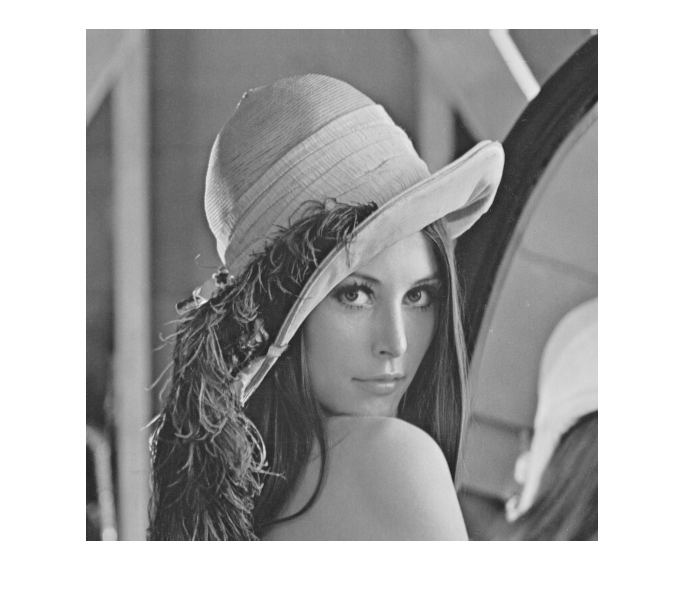
\includegraphics[scale=0.12]{figs/lena.png}}
        \]
        \item The storage cost for $A$ is $mn$ bytes

        \item If we decompose it as $A = USV^T$, then we the cost is $mm + nn + r $ bytes

    \end{itemize}

\vspace{3mm}
\question{
How can we use SVD to save on memory cost?
}

    
\end{frame}


\begin{frame}{Compression with SVD}
\begin{itemize}
    \item Notice what $A=USV^T$ looks like:
\[
    A = \sigma_1 u_1 v_1^T + \sigma_2 u_2 v_2^T + \dots + \sigma_r u_r v_r^T +
0u_{r+1}v_{r+1}^T + \dots + 0u_{p} v_{p}^T
\]

\item This is easily truncated to
\[
    A = \sigma_1 u_1 v_1^T + \sigma_2 u_2 v_2^T + \dots + \sigma_r u_r v_r^T
\]
\item We can discard useless eigenvectors: 
\[
A =
\underbrace{
\begin{bmatrix}
    | &  & | \\
    u_1    & \dots  & u_m \\
    | &   & |
\end{bmatrix}}_{\textrm{keep $r$ columns}}
\begin{bmatrix}
    \sigma_1 &        &          &        &\\
             & \ddots &          &        & \\
             &        & \sigma_r &        & \\
             &        &          & \ddots & \\
             &        &          &        & 0 
\end{bmatrix}
\underbrace{
\begin{bmatrix}
    - & v_1^T & -\\
     & \vdots & \\
    - & v_n^T & -
\end{bmatrix}}_{\textrm{keep $r$ rows}}
\]

\end{itemize}

% What are the savings?  
% \begin{itemize}
%     \item $A$ takes $m\times n$ storage
%     \item Using $k$ terms of $U$ and $V$ takes $k(1 + m + n)$ storage
% \end{itemize}
\end{frame}

%%%%%%%%%%%%%%%%%%%%%%%%%%%%%%%%%%%%%%%%%%%%%%%%%%%%
\begin{frame}{Memory Savings}

\begin{block}{Storage Cost Comparison}
\begin{itemize}
    \item Original matrix \( A \in \mathbb{R}^{m \times n} \):  
    \[
    \text{Cost: } mn \text{ bytes}
    \]
    \item If $r=\rank A$ then   

    \[
    \text{Cost: } r(m + n + 1) \text{ bytes}
    \]
\end{itemize}
\end{block}

\vspace{3mm}
\begin{itemize}
    \item We can compress \emph{more aggressively} 
    \item Keep only the top $k$ singular values $\sigma_1, \ldots, \sigma_k$
\end{itemize}
\end{frame}


%%%%%%%%%%%%%%%%%%%%%%%%%%%%%%%%%%%%%%%%%%%%%%%%%%%%%%%%%%%%%%%


\begin{frame}{Deleting Singular Values}
\begin{itemize}
    \item Choose some integer $k < \rank A$
    \item We can discard least important singular values 
\[
A =
\underbrace{
\begin{bmatrix}
    | &        & |  &    &         \\
    u_1 & \cdots & u_k & 0 & \cdots \\
    | &        & |  &    &         
\end{bmatrix}}_{\text{keep $k$ columns}}
\begin{bmatrix}
    \sigma_1 &          &          &        &         \\
             & \ddots   &          &        &         \\
             &          & \sigma_k &        &         \\
             &          &          & 0      &         \\
             &          &          &        & \ddots
\end{bmatrix}
\underbrace{
\begin{bmatrix}
    - & v_1^T & - \\
      & \vdots &   \\
    - & v_k^T & - \\
    - & 0     & - \\
      & \vdots &  
\end{bmatrix}}_{\text{keep $k$ rows}}
\]

\item Cost is   $ k(m + n + 1)$ bytes
\end{itemize}
\end{frame}

%%%%%%%%%%%%%%%%%%%%%%%%%%%%%%%%%%%%%%%%%%%%%%%%%%%%
\begin{frame}{Compression Example}
\begin{itemize}
    \item In Matlab,  \texttt{[U, S, V] = svd('lena.bmp')} 
    \item Uncompressed 512 by 512 image file: 262144
    \item Out of the 512 singular values... keep only 50 
    \item Compressed image: 50*(512 + 512 + 1) =  51250
    \begin{center}
        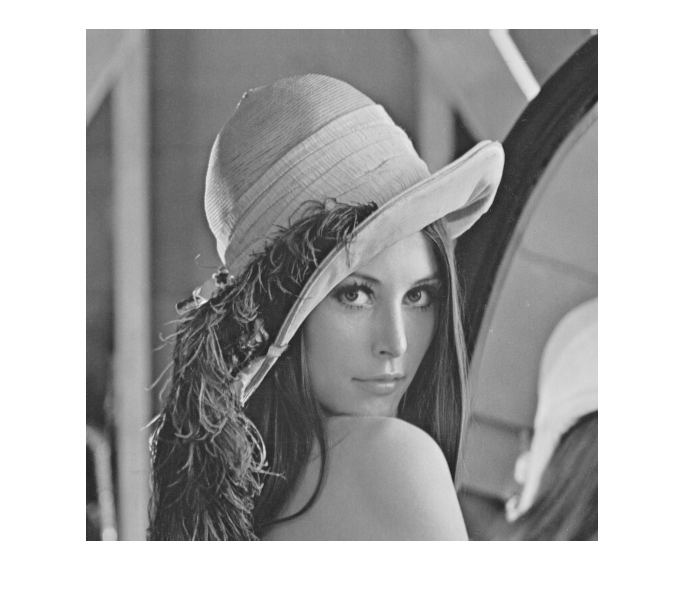
\includegraphics[width=4cm]{figs/lena.png} 
        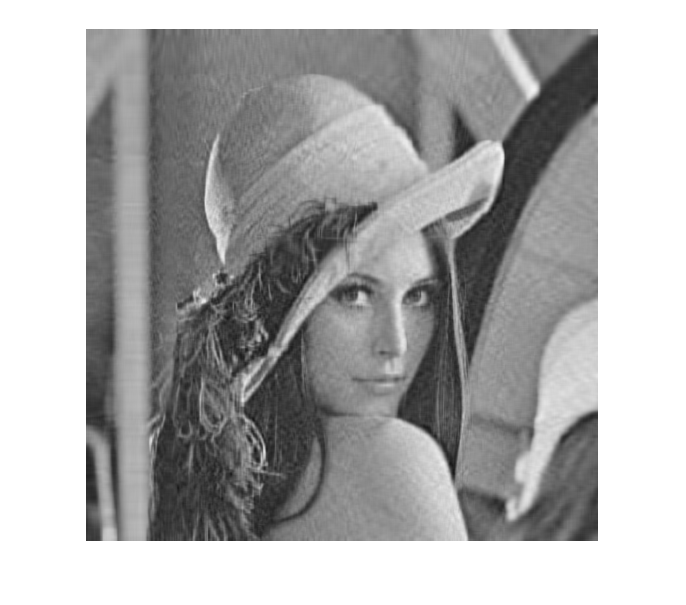
\includegraphics[width=4cm]{figs/lena_compressed.png}
    \end{center}
    \item Compressed image is roughly 20\% of the original 
\end{itemize}
\end{frame}

%%%%%%%%%%%%%%%%%%%%%%%%%%%%%%%%%%%%%%%%%%%%%%%%%%
\begin{frame}{Analogy}

\begin{figure}
    \centering
    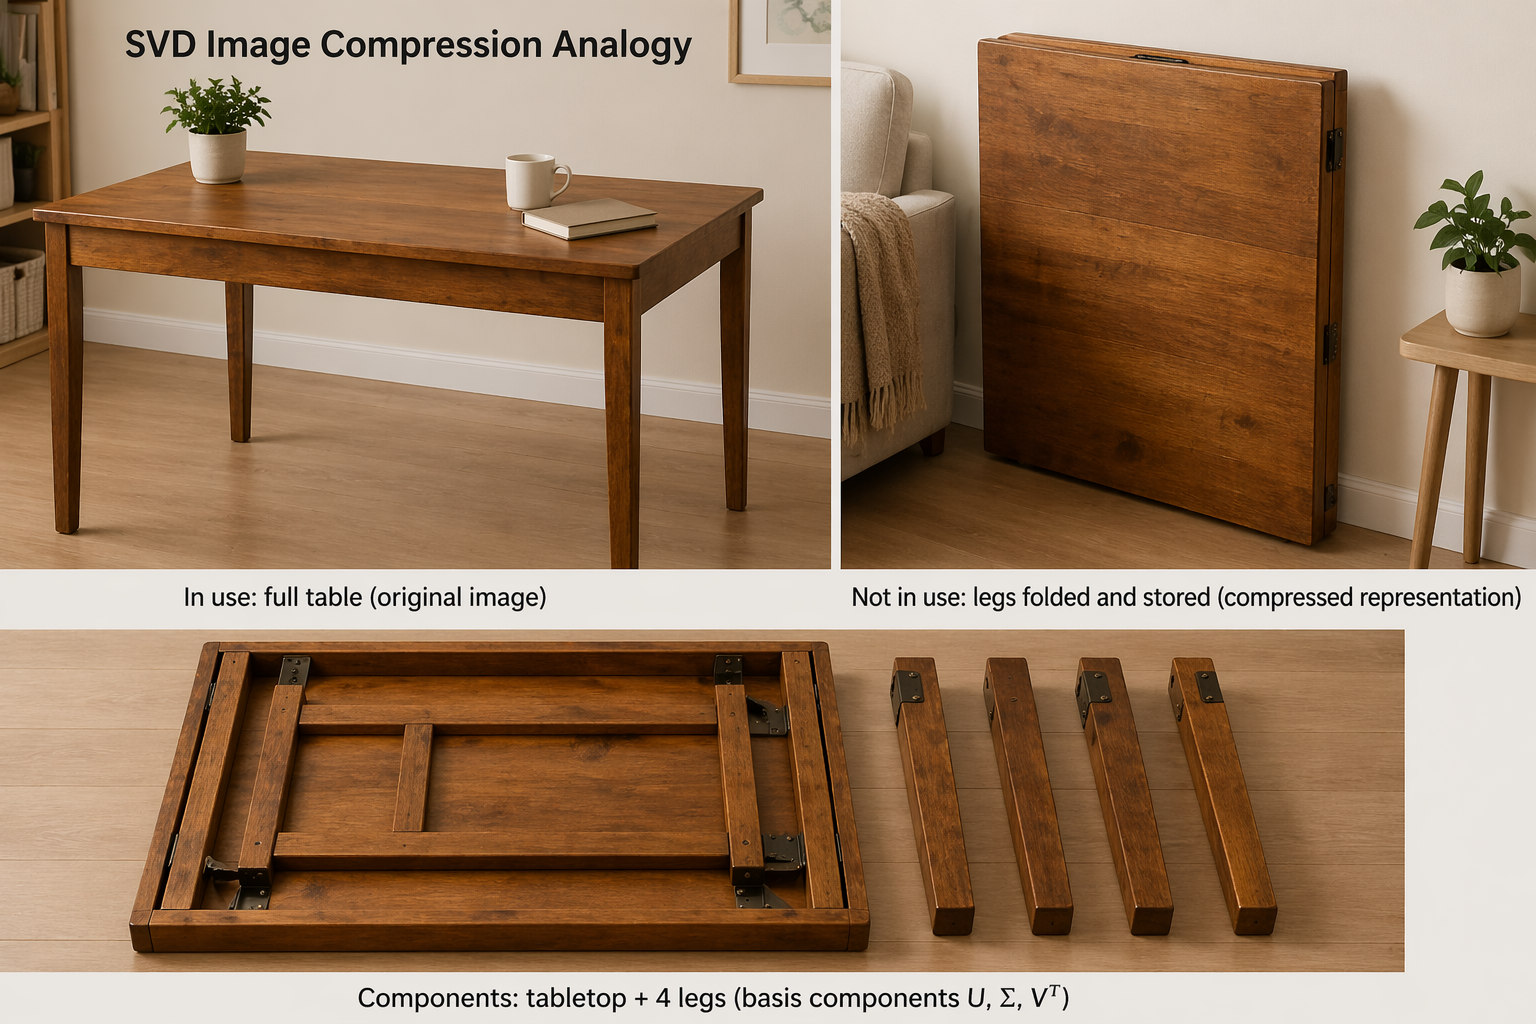
\includegraphics[width=0.8\linewidth]{figs/svd_analogy.png}
    \caption{Using SVD to compress an image is like breaking off the legs and converting it to a fold-out table.}
\end{figure}
    
\end{frame}


\begin{frame}{Deep Fried}
\begin{center}
    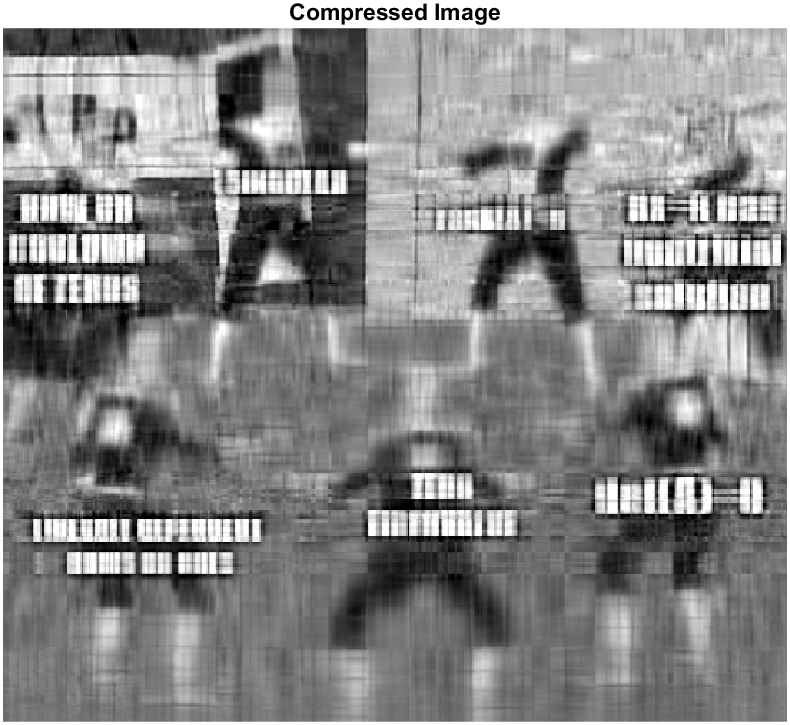
\includegraphics[scale=0.5]{figs/meme-compressed.png}
\end{center}
\end{frame}



\end{document}
